% \documentclass{article}
\documentclass[acmlarge, review=false, screen=true]{acmart}

\usepackage[utf8]{inputenc} 
\usepackage{natbib}
% \usepackage{a4wide}
\usepackage{url}

\citestyle{acmnumeric}
\bibliographystyle{ACM-Reference-Format}

\AtBeginDocument{%
  \providecommand\BibTeX{{%
    \normalfont B\kern-0.5em{\scshape i\kern-0.25em b}\kern-0.8em\TeX}}}

%% Rights management information.  This information is sent to you
%% when you complete the rights form.  These commands have SAMPLE
%% values in them; it is your responsibility as an author to replace
%% the commands and values with those provided to you when you
%% complete the rights form.
% \setcopyright{acmcopyright}
\setcopyright{none}
% \copyrightyear{2018}
% \acmYear{2018}
% \acmDOI{10.1145/1122445.1122456}
\acmDOI{} % This was required so I left it empty    /Casper


%%
%% These commands are for a JOURNAL article.
% \acmJournal{POMACS}
% \acmVolume{37}
% \acmNumber{4}
% \acmArticle{111}
% \acmMonth{8}

% Some of these couldn't be empty, they default to 1    /Casper

\begin{document}


\title{Project report - Postmor}

\author{Alexander Andersson}
\affiliation{%
	\institution{Mälardalen University}
	\city{Västerås} }
\author{Casper Andersson}
\affiliation{%
  \institution{Mälardalen University}
  \city{Västerås} }
\author{Emil Elfström}
\affiliation{%
\institution{Mälardalen University}
\city{Västerås} }
\author{Nick Grannas}
\affiliation{%
  \institution{Mälardalen University}
  \city{Västerås} }
\author{Philip Karlsson}
\affiliation{%
  \institution{Mälardalen University}
  \city{Västerås} }




\maketitle
  \section{Introduction}
    \textcolor{red}{[Introduction] [CA]} \newline
    This is the project report for the development of the Android application Postmor developed for the course DVA232, Programming Mobile Applications, examined by Afshin Ameri. Our application tries to challenge the always online mentality by allowing users to send letters that imitate the physical mail system. Mail is picked up and delivered on set times and takes some time to reach their destination. Our goal for the course is to get grade five. This report describes our work process, problems we encountered and how we overcame them, discuss the results, and suggests improvements and additions that we would like to do if we were to continue the development.

  \section{Background}
    \textcolor{red}{[Description of the application Postmor] [PK]} \newline
    Postmor is an application for sending handwritten letters in a manner that imitates physical mail. The user writes a letter on paper and sends it via the app. The letters are routed from the recipient’s unique “home address”; which is chosen when signing up. The emptying of post-boxes is done on set times each day and delivery takes 48 hours. Postmor provides a “new” medium for communication without the pressure to reply quickly. Just like sending real letters there is time to sit down and compose an answer. The users will have a sense of accomplishment after sending a letter and will be delightfully surprised when they receive a letter. The target audience is those interested in the charm of old fashioned mail. The barrier of entry is low compared to sending physical mail (buying envelopes, stamps, getting the address, and putting the letter in the mailbox).

  \section{Related works}
    \textcolor{red}{[Related works] [NG]} \newline
    Slowly is an application that is used to send letters between users\cite{slowly}. The application uses stamps as one of their gimmicks. You receive one or two stamps that correlate to your country. In the app, you can collect stamps from other users. Another gimmick is that delivery times are dependent on the distance between countries. In Slowly you are notified when a letter is incoming and how long until it arrives as well as your send and received ratio. You also have a profile page where you can list your interests as well as a biography. The app also features a matchmaking system where you can find other users depending on your interests or if you would like to to be contacted by anyone that is looking for a penpal.

    \textcolor{red}{[Activities] [CA]} \newline
    Activities are the foundation of Android applications\cite{activity}. They create the initial window where all other UI components live. An application requires at least one activity. There can be many activities that stack on each other or they can be embedded in other activities. 

    \textcolor{red}{[Fragments] [CA]} \newline
    Fragments are similar to activities and can contain the same things and have their own behavior\cite{fragments}. However, they must be placed inside an activity or inside another fragment. The fragment’s lifecycle is dependent on the activity it is placed inside. If the activity dies it kills all the fragments inside it.

    \textcolor{red}{[ViewModel data sharing] [EE]} \newline
    A ViewModel is a class that is designed to store and manage UI data\cite{viewmodel}. ViewModels are life-cycle aware and survive configuration changes such as screen rotation, as opposed to fragments and activities that will be destroyed and recreated. This makes ViewModels ideal for storing persistent data and sharing data between fragments. To easily share data between fragments they first need to share the same ViewModel. A server request will then update a live data variable in the ViewModel. Any fragment that is observing that data for changes will then automatically receive the newly updated data and can immediately reflect these changes in the user interface. 

  \section{Objectives and goals}
    \textcolor{red}{[About the target audience] [PK]} \newline
    We have identified a few of our target audiences: Hipsters, teachers, and the elderly. We imagine a typical user from each group to identify their potential needs. We think hipsters would like Postmor because it differs from mainstream messaging applications. Teachers could use Postmor to teach writing. Schools across the globe could partner up and have the students be pen-pals. The elderly will enjoy the nostalgic experience of receiving handwritten letters and taking the time to read and carefully compose letters. They could also use it to communicate with their grandchildren. 

    \textcolor{red}{[The main objective] [PK]} \newline
    Postmor is also a homage to the elderly and the way things were done before. Research shows that innovation should not dismiss the wisdom of the past\cite{design-inspiration}. Postmor aims to mend that. The most striking difference between Postmor and mainstream communication apps might be the absence of information about incoming messages. The user can be certain that their letter will be delivered. What they don’t know is whether messages are on the way to them, or if their sent messages have been read. This is intentional and mimics how real mail works. This absence of information allows the user to focus on the correspondence and take their time reading and writing letters. Research shows that such a minimalistic design leads to new interaction techniques\cite{simplicity-in-interactiondesign}, which we think will be less stressful for users.

    \textcolor{red}{[Overarching goals] [PK]} \newline
    Our goals were:
    \begin{itemize}
      \item Achieve a functional service for sending messages with all core features implemented.
      \item No bugs or crashes resulting in permanent loss of user data. 
      \item The server is scalable and ready to handle additional users and correspondence. 
      \item No unexpected behavior. 
    \end{itemize}

    This satisfies the requirement for grade 5 that the app should be ready for release.

  \section{Project plan}
      \begin{figure}
      % \includegraphics[width=\textwidth]{images/screenshot-of-WKC.png}
      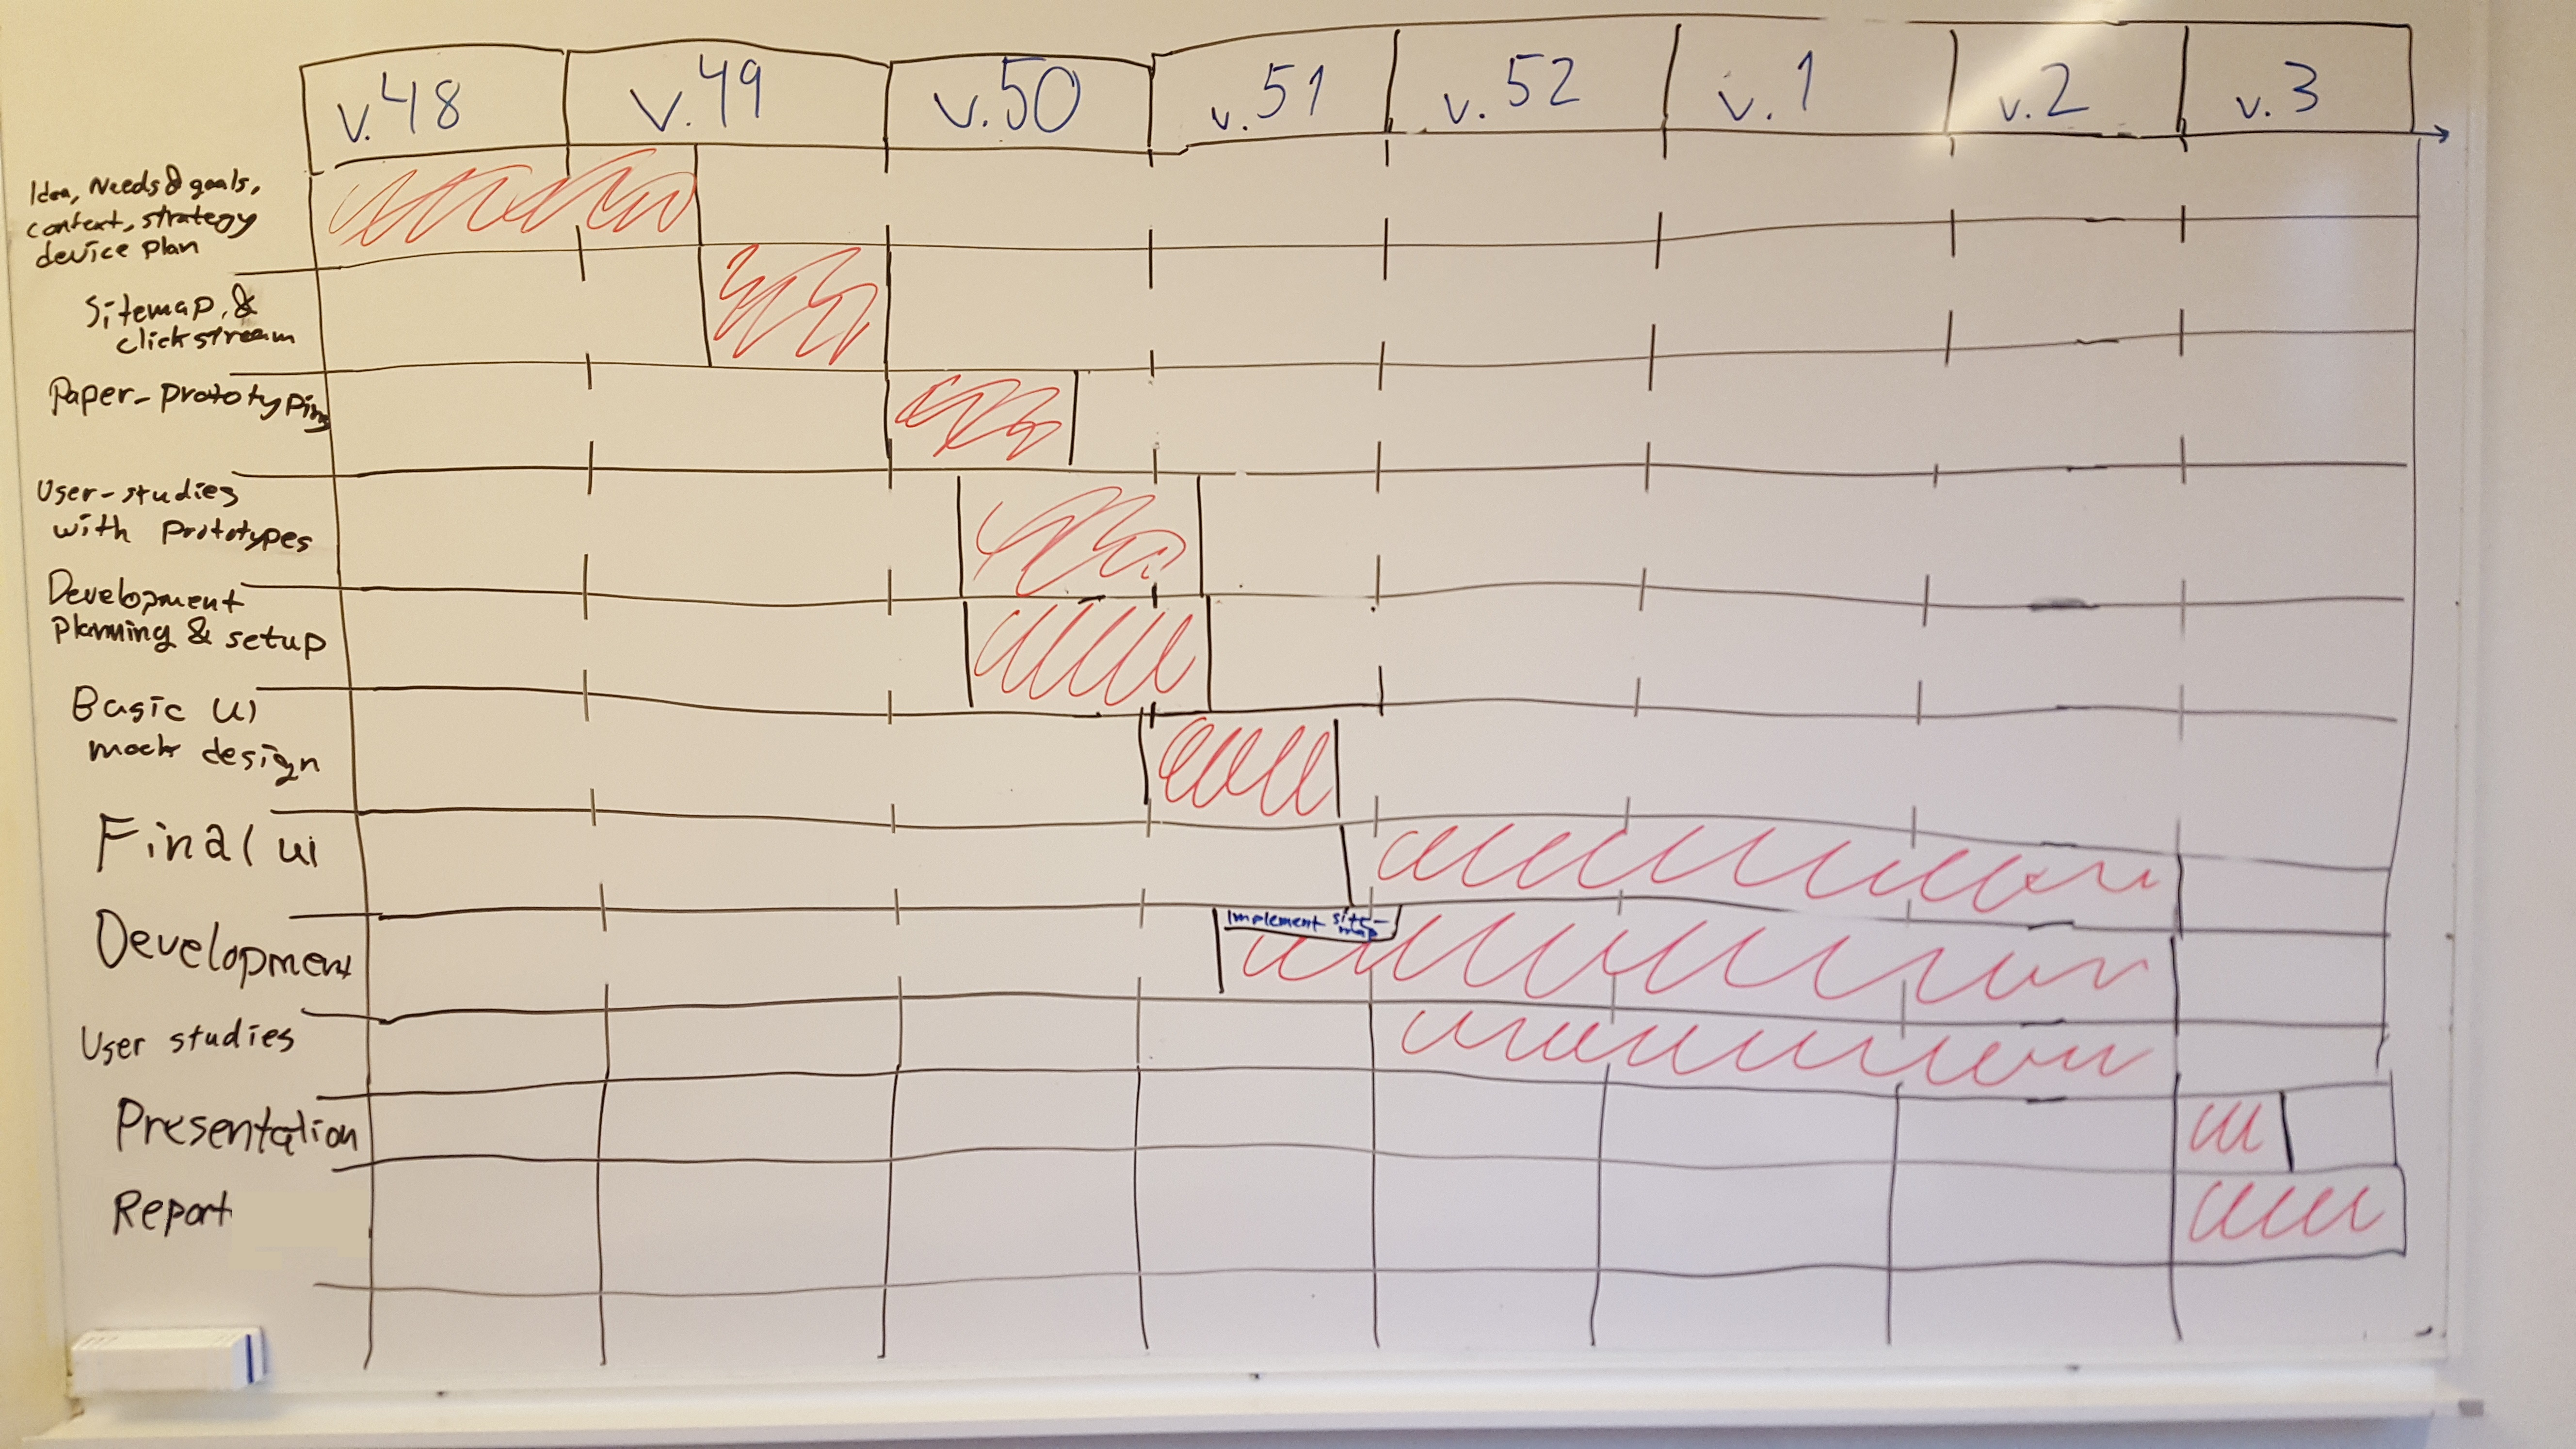
\includegraphics[width=\textwidth]{images/Gantt_schema.jpg}
      \Description{Gantt}
      \caption{Gantt chart}
      \label{fig:gantt}
    \end{figure} 
    \textcolor{red}{[How we planned the project] [PK]} \newline
    After the specifications, objectives, and goals for Postmor were established, we planned the project. Our business student consultant Fredrik helped construct a Gantt chart\cite{gantt} as seen in fig. \ref{fig:gantt}. We based the procedure of the planning-template described by Afshin Ameri in a lecture for this course\cite{lecturenotes-mobile}. Based on our experience from the course “Development of web applications”. We planned to do the design work early to have plenty of time for coding. This way we would have time to test a finished product.

    \textcolor{red}{[Why we planned it like this] [PK]} \newline
    Experience from previous courses tells us that if we do not put enough care into the design phase, the implementation will be more difficult. To avoid a disorganized codebase we spent the first week and a half solely discussing the app’s functionality. That way each of us would have the same vision (as far as it is possible). We then built a sitemap, a clickstream, and made several iterations of paper prototypes\cite{lecturenotes-mobile}. Because of this thorough groundwork, there were few big problems due to misunderstandings during the development phase.


  \section{Problems}

    \subsection{Supporting different screen sizes}
      \begin{figure}
        % \includegraphics[width=\textwidth]{images/screenshot-of-WKC.png}
        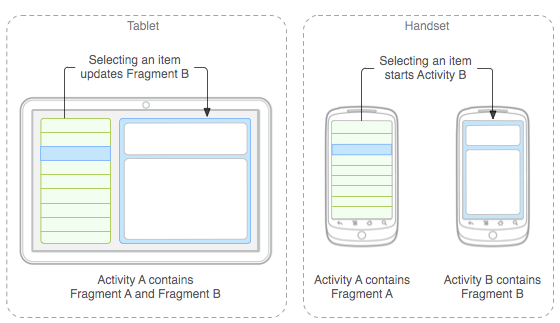
\includegraphics[width=\textwidth]{images/FRAGMENTS.png}
        \Description{Tablet view}
        \caption{Tablet example}
        \label{fig:tablet-view}
      \end{figure}

      \textcolor{red}{[The plan was to have multiple fragments in view] [PK]} \newline
      Initially, we decided to have different designs for phones and tablets. The main difference for tablets was the box screen, where we wanted the messages in a list to the left and the content of the selected message displayed on the right (fig. \ref{fig:tablet-view}). This design would make use of the larger screen area to provide a better user experience. However, tablets currently make up less than 5\% of the global market\cite{statcounter}. Since most users will be on their phone, we set up that design first. We used the android Jetpack Navigation component to set up the UI-architecture\cite{navigation}. There is one main activity that was configured to switch between different fragments. Androids latest recommendations are to develop single-activity apps\cite{singleactivity}. 

      \textcolor{red}{[Problem with concurrent fragments and the solution] [PK]} \newline
      Towards the end of development, we found that the navigation framework did not support navigation to multiple fragments simultaneously within a single activity. The first option was to refactor the app for multiple activities. This was not feasible considering the time we had, as we would have to learn and master another app structure and apply it to a work in progress application. We went with the second option: Use the same UI-architecture for all screen sizes. We tweaked margins and sizes of different elements in the layout resources that would be used for devices with a width greater than 600 density-independent pixels. 

      \textcolor{red}{[Why a similar tablet navigation graph is good] [PK]} \newline
      We concluded that having several fragments in one view had been too highly prioritized. Our users would spend most of the time using our app with pen and paper. The increased productivity provided by the message list on the left and the content of the chosen message on the right might be useful in an email application but is not essential for longer letters. 

    \subsection{Data sharing between app components}
      \textcolor{red}{[Problem with connecting fragments] [EE]} \newline
      When the development phase began we realized that communication between components works differently than what we were used to since we decided to use the multiple fragment approach. Fragments should be self-contained and never directly communicate with other fragments\cite{fragmentcommunication}, which means that fragments will always be unaware of each other. Since fragments never have a connection to each other it would not be possible for us to send data directly between different fragments.

      \textcolor{red}{[Solving data sharing with ViewModels] [EE]} \newline
      There are two main methods to solve the issue with fragment communication. The first method is to communicate through the activity that all the fragments are associated to. The second method is to use a shared ViewModel. We decided to use ViewModels since we could have different ViewModels for different parts of the app, which allowed for better separation of concerns. This way we could also separate stored data from UI logic since ViewModels are not affected when fragments are interrupted or destroyed\cite{viewmodel}. The fragments can also be completely unaware of each other even if they use the same ViewModel.



      \begin{figure}
        % \includegraphics[width=\textwidth]{images/screenshot-of-WKC.png}
        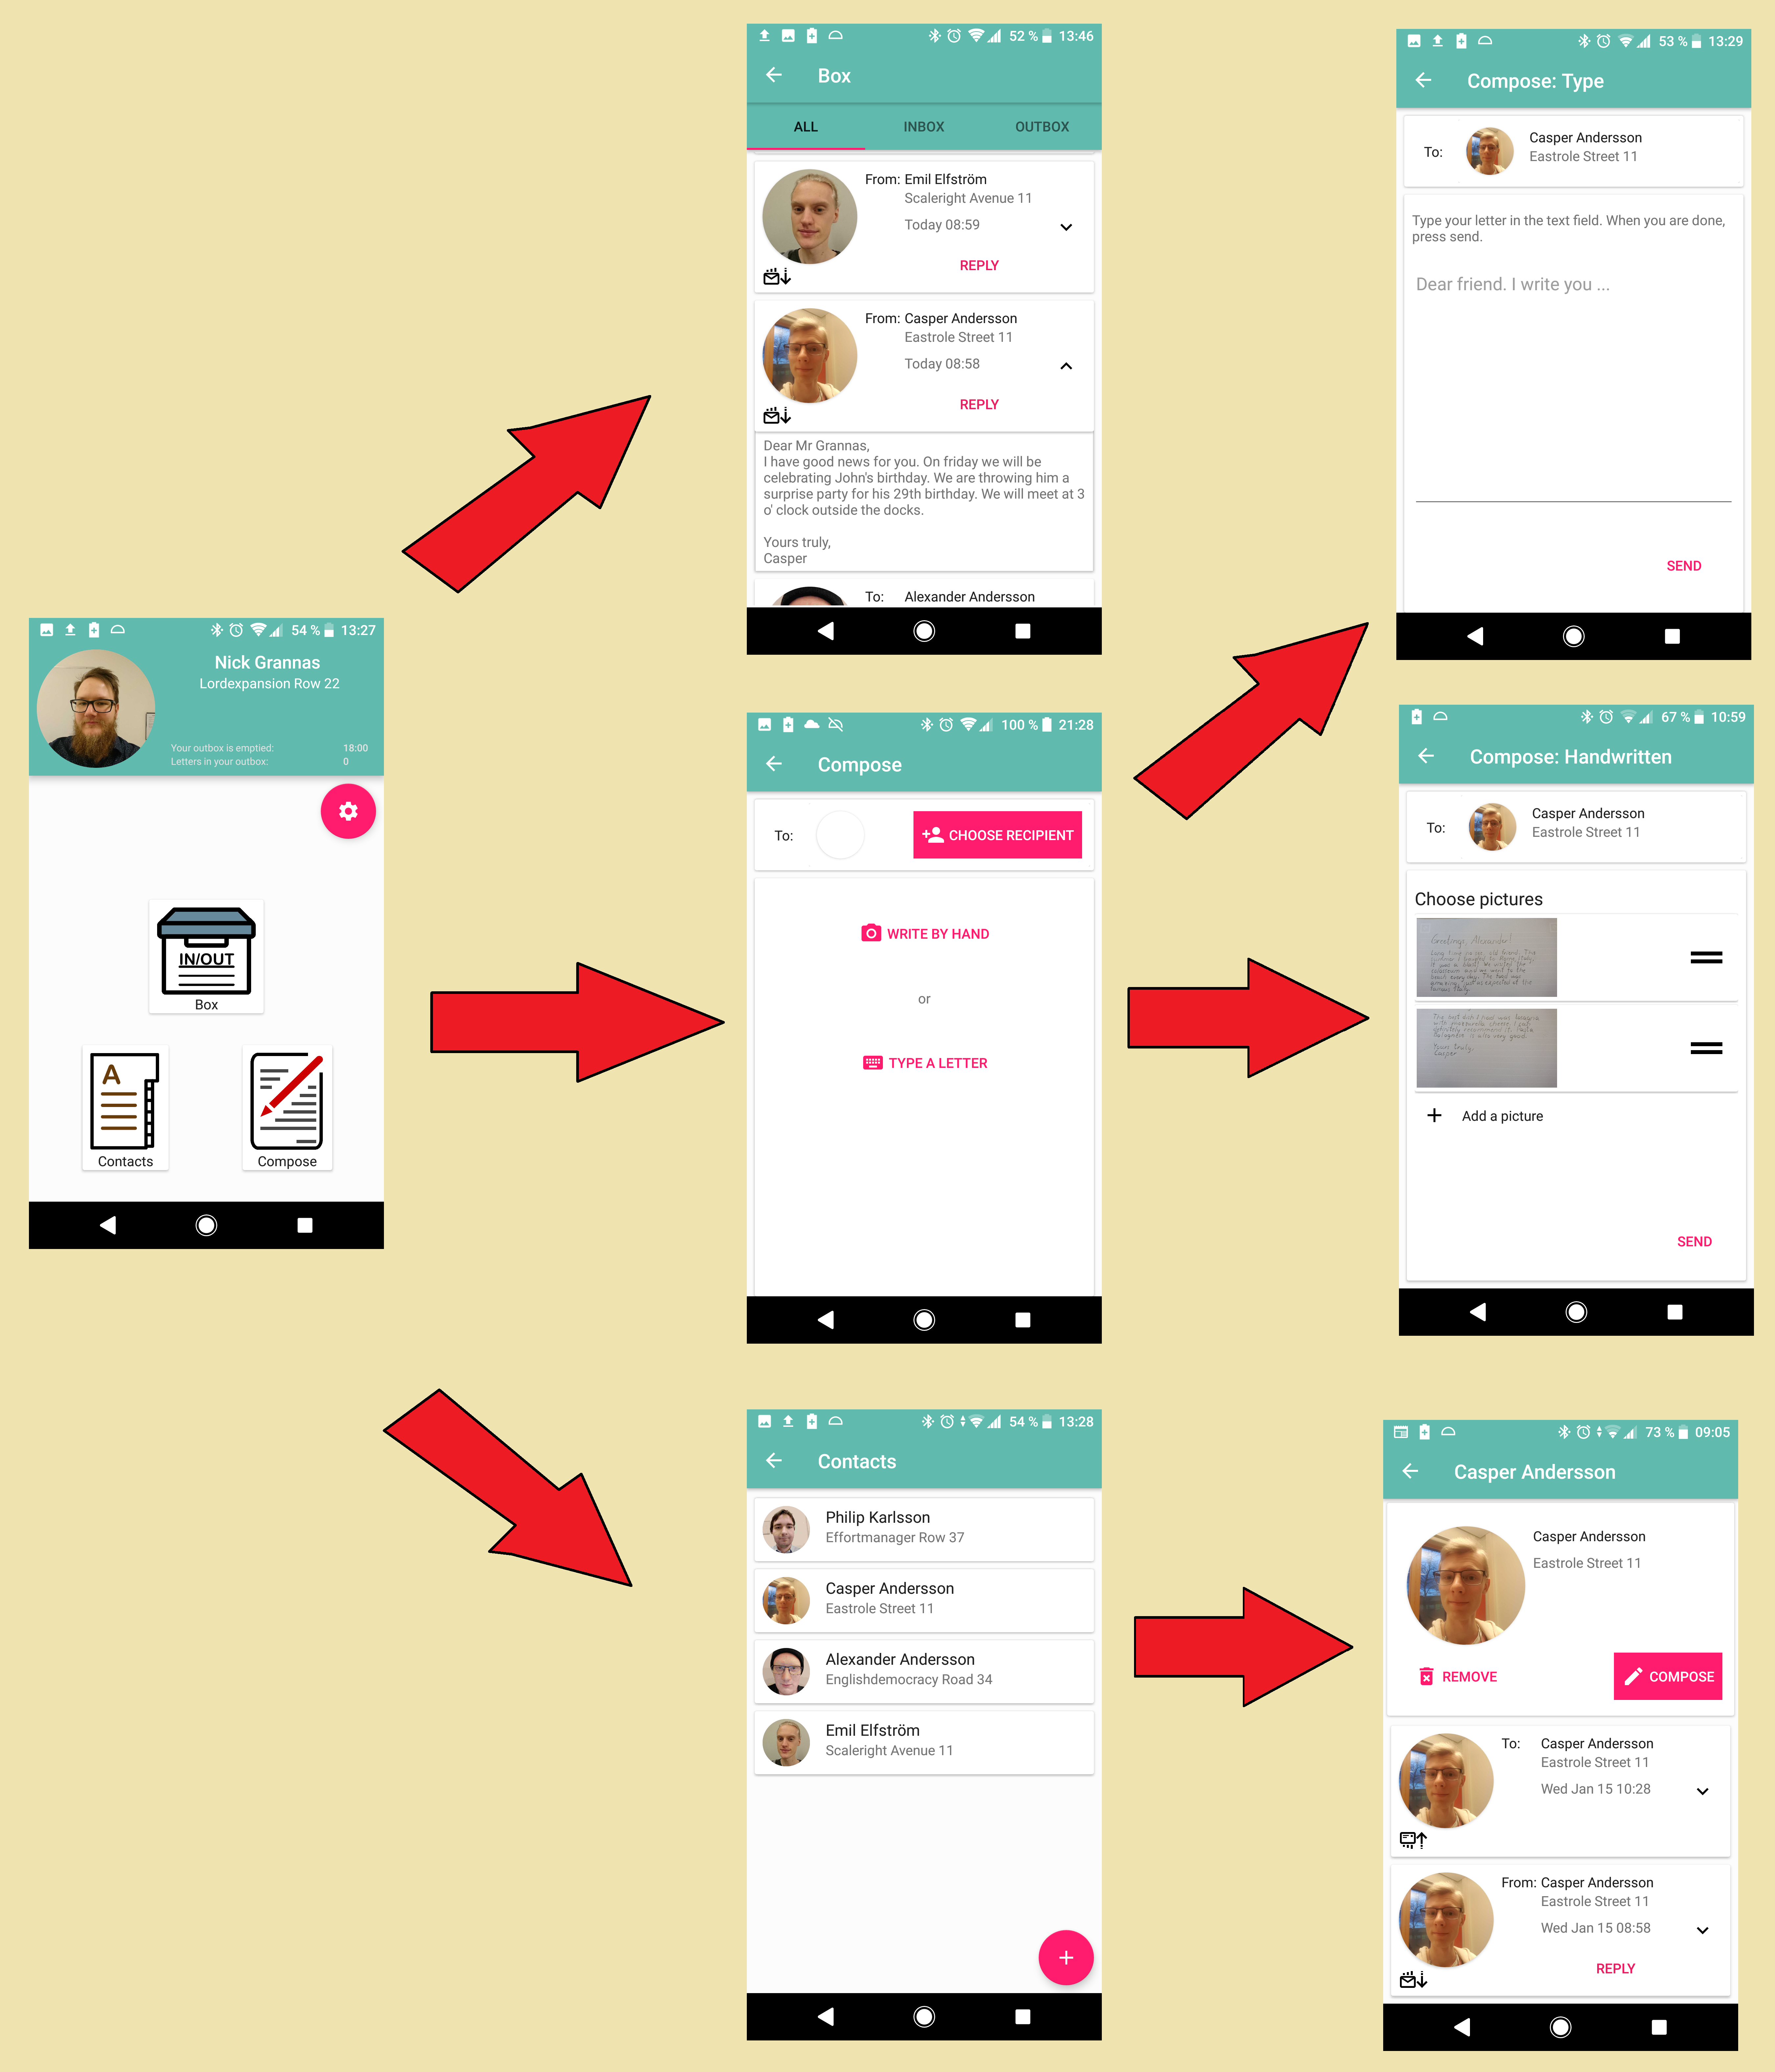
\includegraphics[width=10cm]{images/Simplified_structure.png}
        \Description{Simplified view}
        \caption{A simplified version of the app’s structure.}
        \label{fig:simplified-nav}
      \end{figure}
    \subsection{Fetching data}
      \textcolor{red}{[The problems with fetching all data at once] [CA]} \newline
      Towards the end of the project, we realized a problem with fetching data from the API. When a user logs in for the first time on the app, all contacts and messages are fetched from the server. Since the response contains lots of images it could be large. The parsing of large Base64 strings always took several seconds. Because Java parsing limitations only one depth level could be parsed at a time, meaning that any nested data was parsed multiple times. We later learned that many other groups connected their app directly to a remote database, not using a web API. That solution wouldn’t have required JSON parsing and could have saved time. However, our solution was to reduce the size of the images. We did this without drastically affecting the details. This improved load times enough to not be a problem. But for a user with hundreds of messages and contacts, this could still cause inconvenience when reinstalling the app or clearing the application cache in Android system settings.


    \subsection{Problems with the database}
      \textcolor{red}{[An oversight in the database schema led to last-minute fixes] [AA]} \newline
      During late development, we encountered a bug that seemed to make contacts disappear. Investigation revealed that multiple users could not have the same user in their address book. This bug was a result of an oversight in the design stage of the database relational schema. In the original schema, the relationship between users and contacts had a one-to-many relationship that should have been a many-to-many relationship. The oversight became apparent when all parts of the project were put together. This bug might have just required a small or moderate fix if found earlier. Due to problems with Entity Framework Core\cite{adodotnet} and artifacts from old database migrations, it instead became a difficult and time-consuming task to fix in time for the presentation.

  
  \section{Results}

    \subsection{Register}
      \textcolor{red}{[Registration process] [NG]} \newline
      When a user uses Postmor for the first time they need to register. We felt that instead of having one single page to put all the information in we wanted to have a lighter feel to it with less information (fig. \ref{fig:register}). The user enters their email which is then used for signing in. They enter their name and a semi-random address is generated for them. If the address is not to their liking they can generate a new one. On the second page the user is presented with a “contact card” where they can upload a profile picture, but choosing a picture is not necessary to complete the registration. Lastly, a password is chosen. The app shows the user which criteria the password must meet to be valid.

      \begin{figure}
        % \includegraphics[width=\textwidth]{images/screenshot-of-WKC.png}
        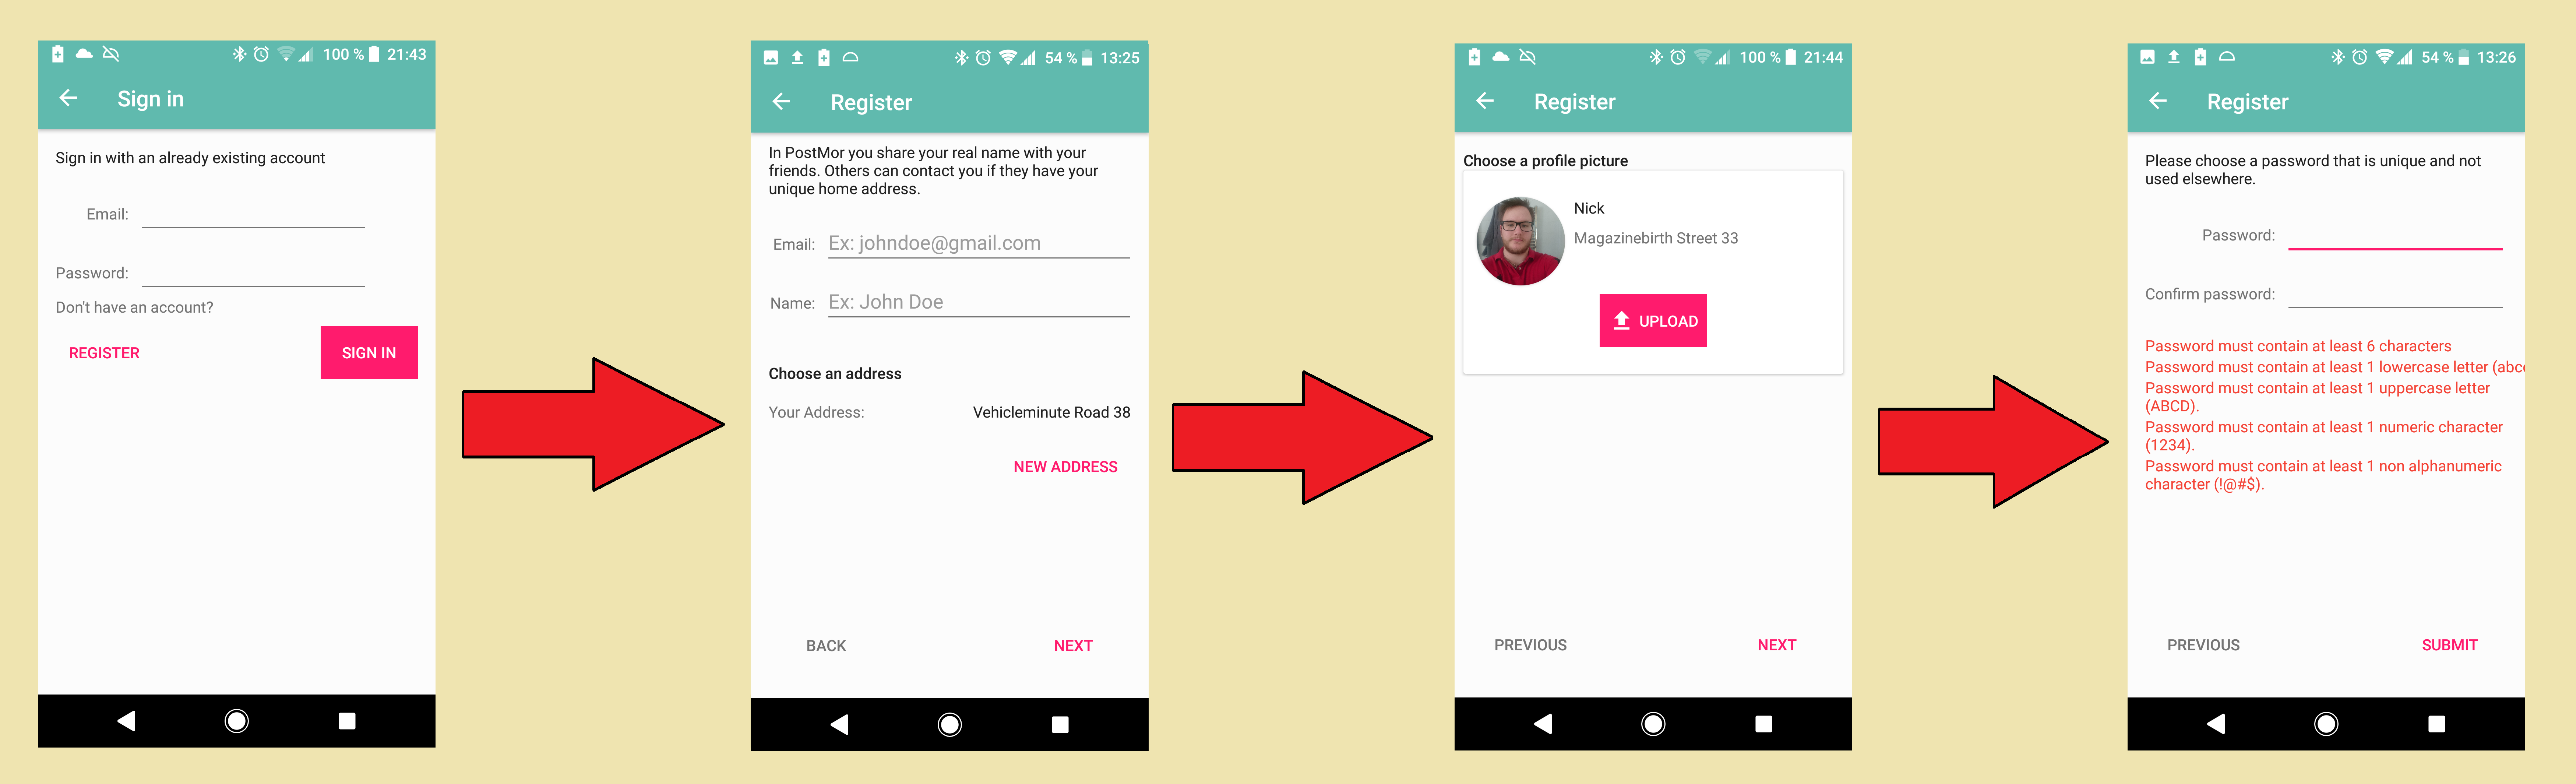
\includegraphics[width=\textwidth]{images/LOGIN-REGISTER.png}
        \Description{Simplified view}
        \caption{An overview of the registration process. Each picture shows what information a user needs to enter.}
        \label{fig:register}
      \end{figure}

    \subsection{Home}
      \textcolor{red}{[Description of the design of the home screen] [NG, PK]} \newline
      The home screen (fig. \ref{fig:home}) greets the user when they first open the app after logging in. All key features are accessible from here. The top shows a profile card that displays the logged-in user’s name, address, and profile picture. It also shows the time when their letters are sent and how many letters are ready to be sent. Three buttons lead to the main screens and a settings button (fig. \ref{fig:simplified-nav}). We wanted the home screen to be the central hub in the app and all the important information should be visible there. The color scheme is light to reinforce our vision of a relaxed user experience. Difference in elevation is used for different layers of elements according to the material design guidelines\cite{materialdesign}. The icons are based on designs by graphic designer Pausrr\cite{pausrr} and have been modified to suit our app.


      \begin{figure}[!tbp]
        \centering
        \begin{minipage}[b]{0.4\textwidth}
          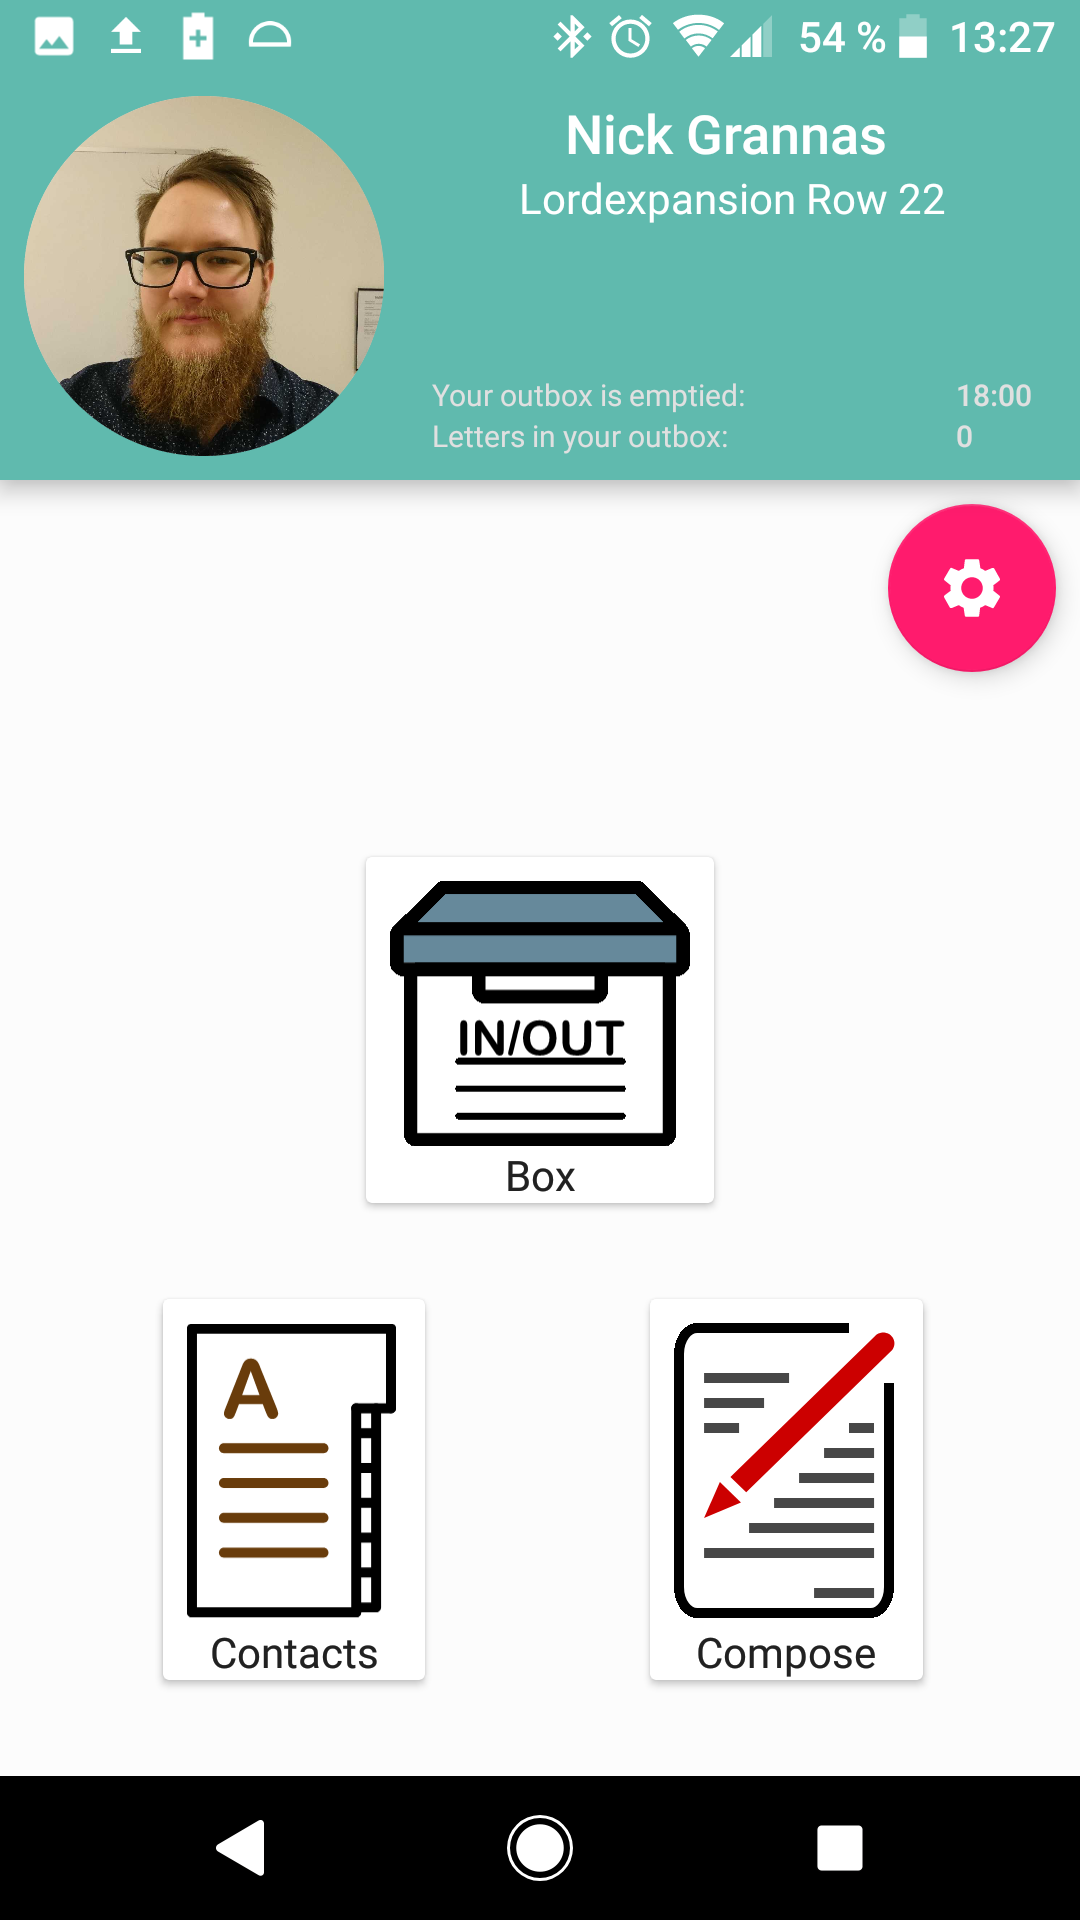
\includegraphics[width=\textwidth]{images/HOME.png}
          \caption{The home screen contains all the necessary actions and information that the user needs. Large buttons make it easy to access each screen.\newline}
          \label{fig:home}
        \end{minipage}
        \hfill
        \begin{minipage}[b]{0.4\textwidth}
          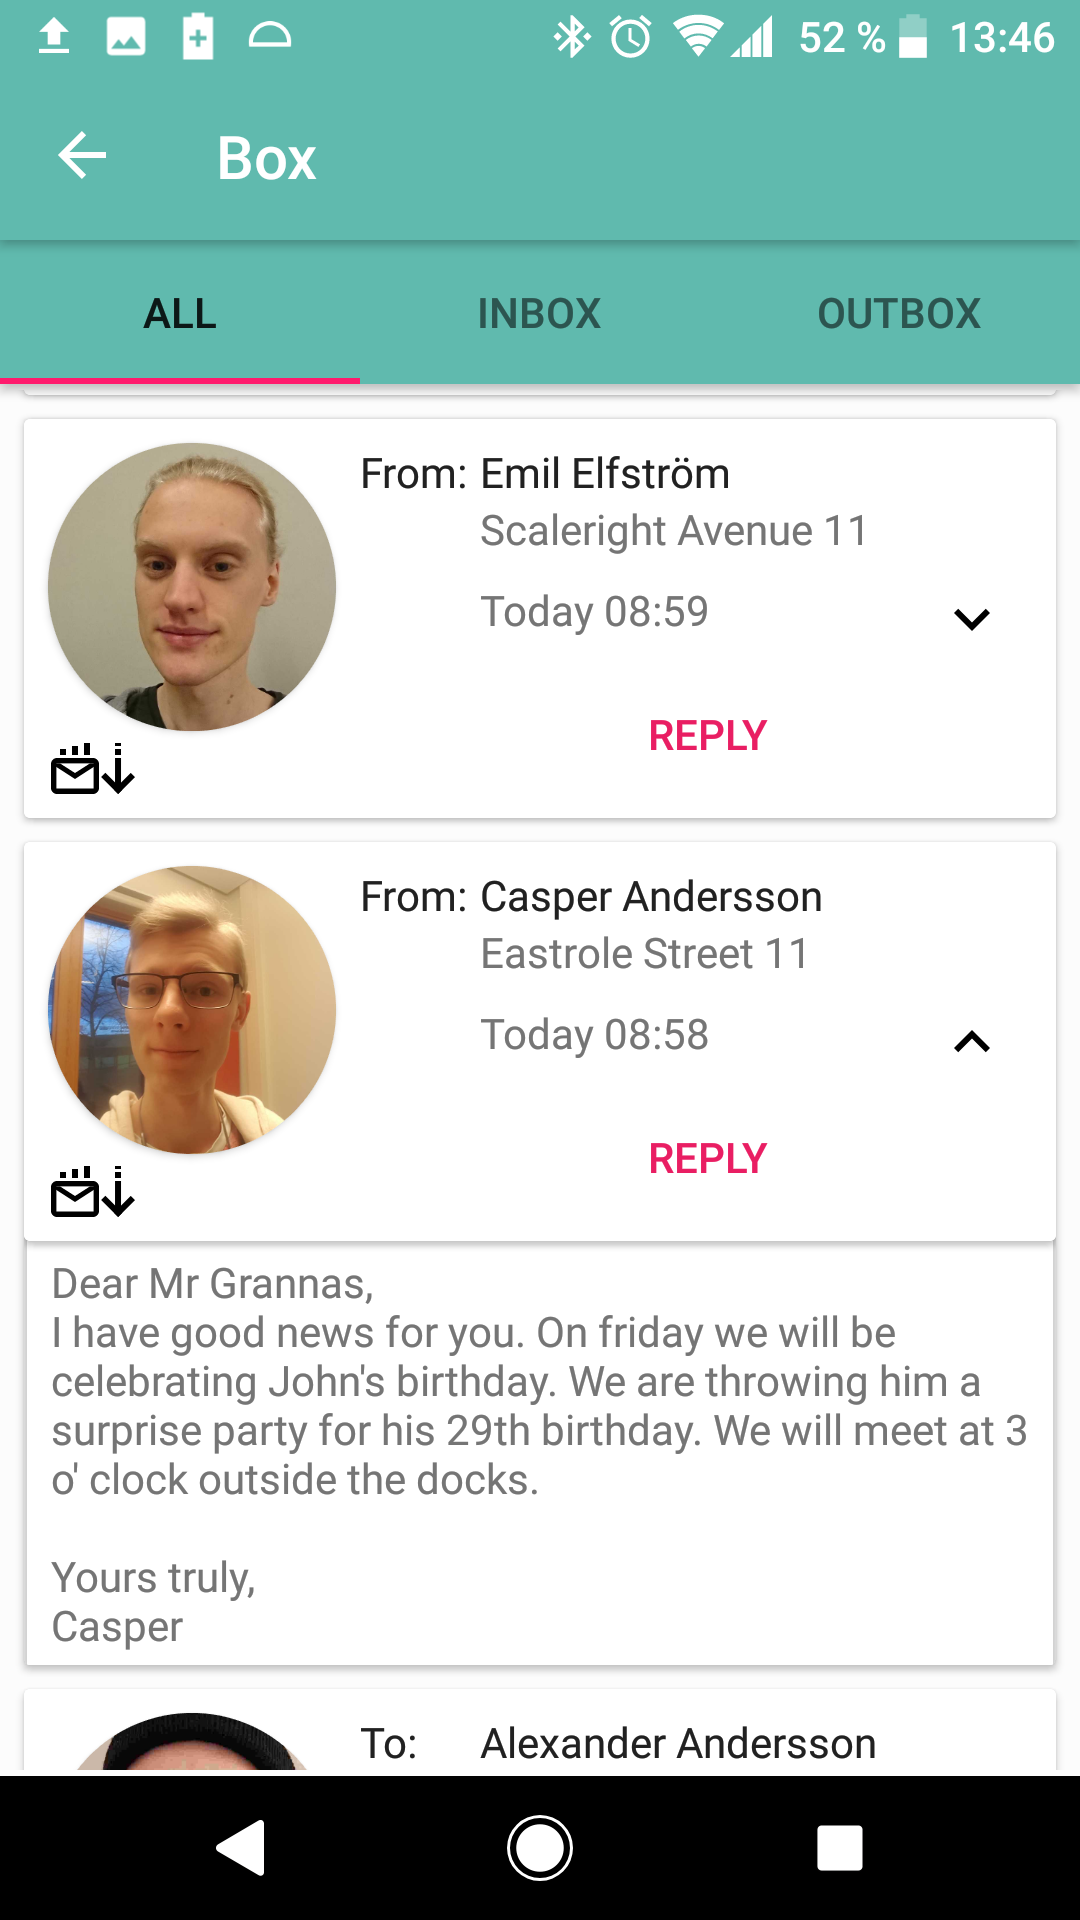
\includegraphics[width=\textwidth]{images/BOX.png}
          \caption{Users can see all the letters received from and sent to their contacts. The tab header indicates which content is displayed in each tab. Letters can easily be viewed and responded to.}
          \label{fig:box}
        \end{minipage}
      \end{figure}

      \begin{figure}[!tbp]
        \centering
        \begin{minipage}[b]{0.4\textwidth}
          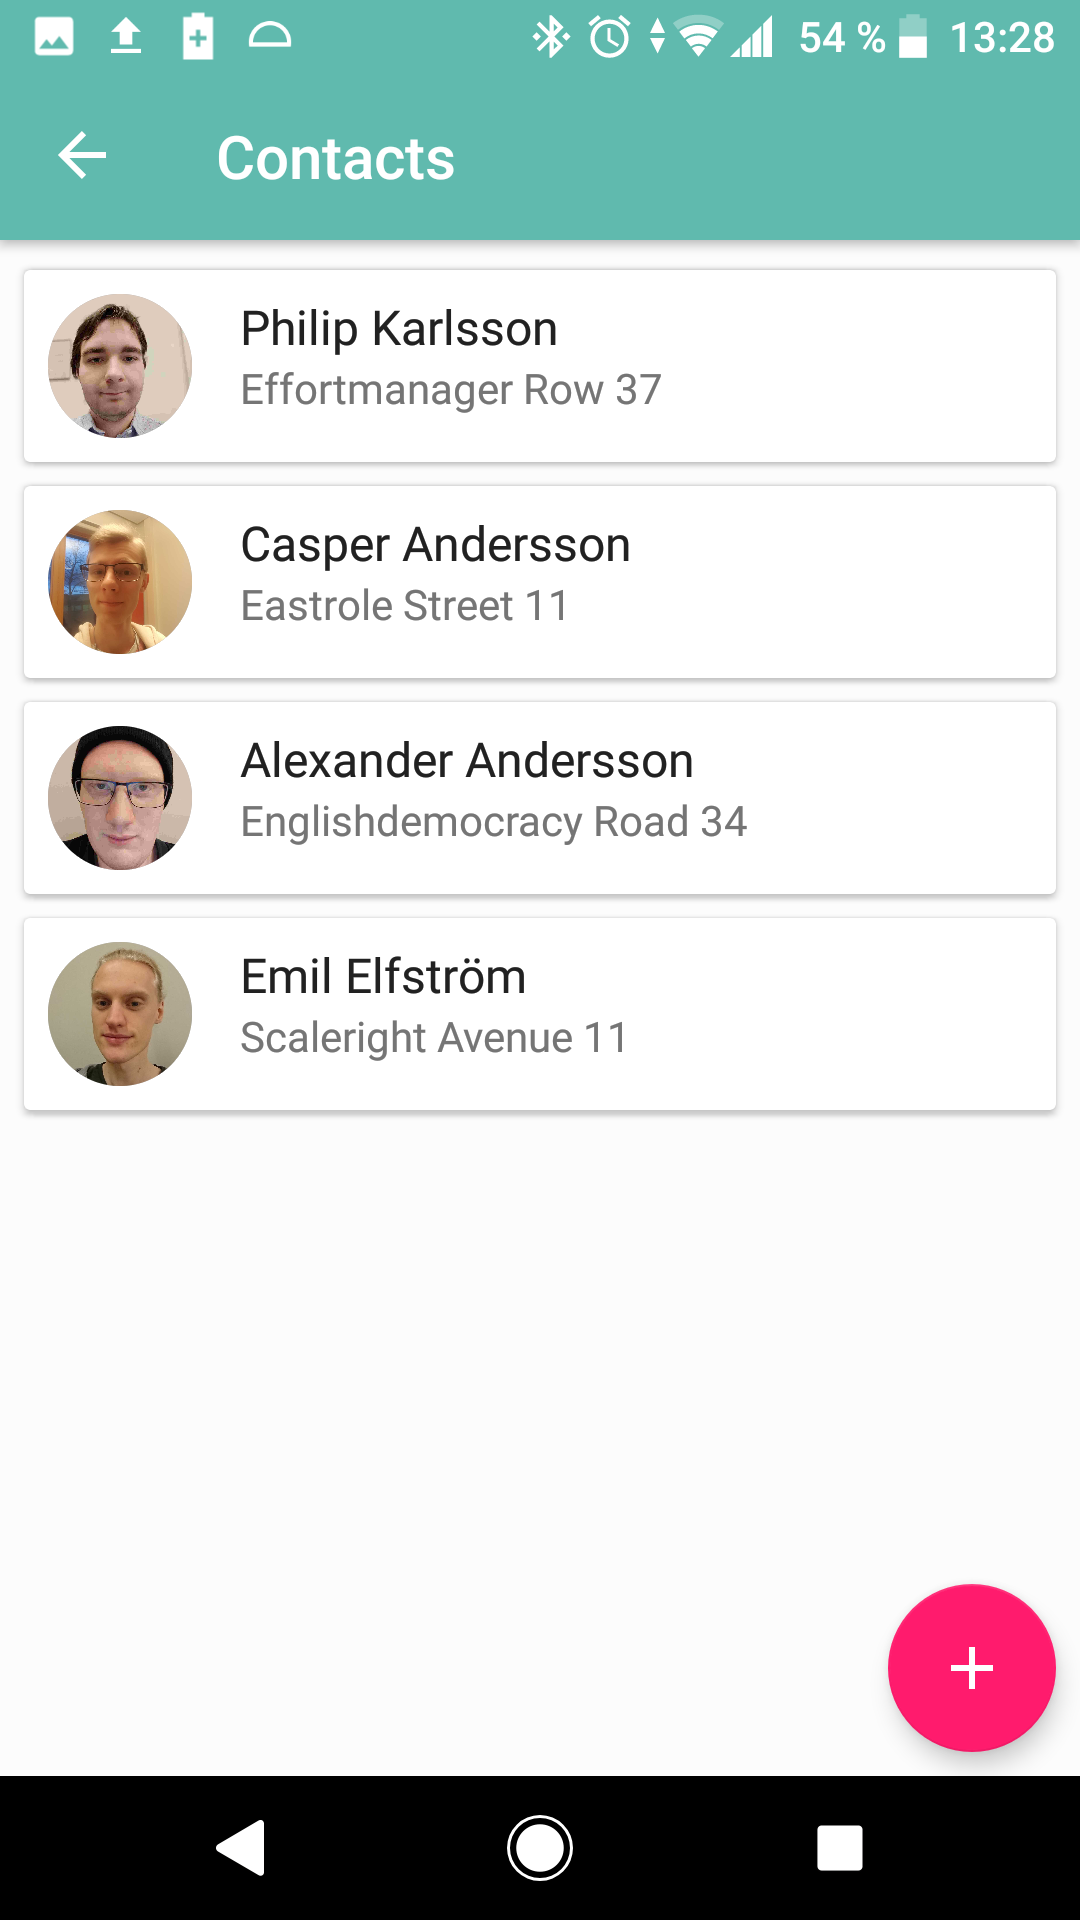
\includegraphics[width=\textwidth]{images/Contacts.png}
          \caption{Contacts shows all your added contacts with their information. In the bottom right corner, there is a button for adding a new contact.\newline \newline}
          \label{fig:contacts}
        \end{minipage}
        \hfill
        \begin{minipage}[b]{0.4\textwidth}
          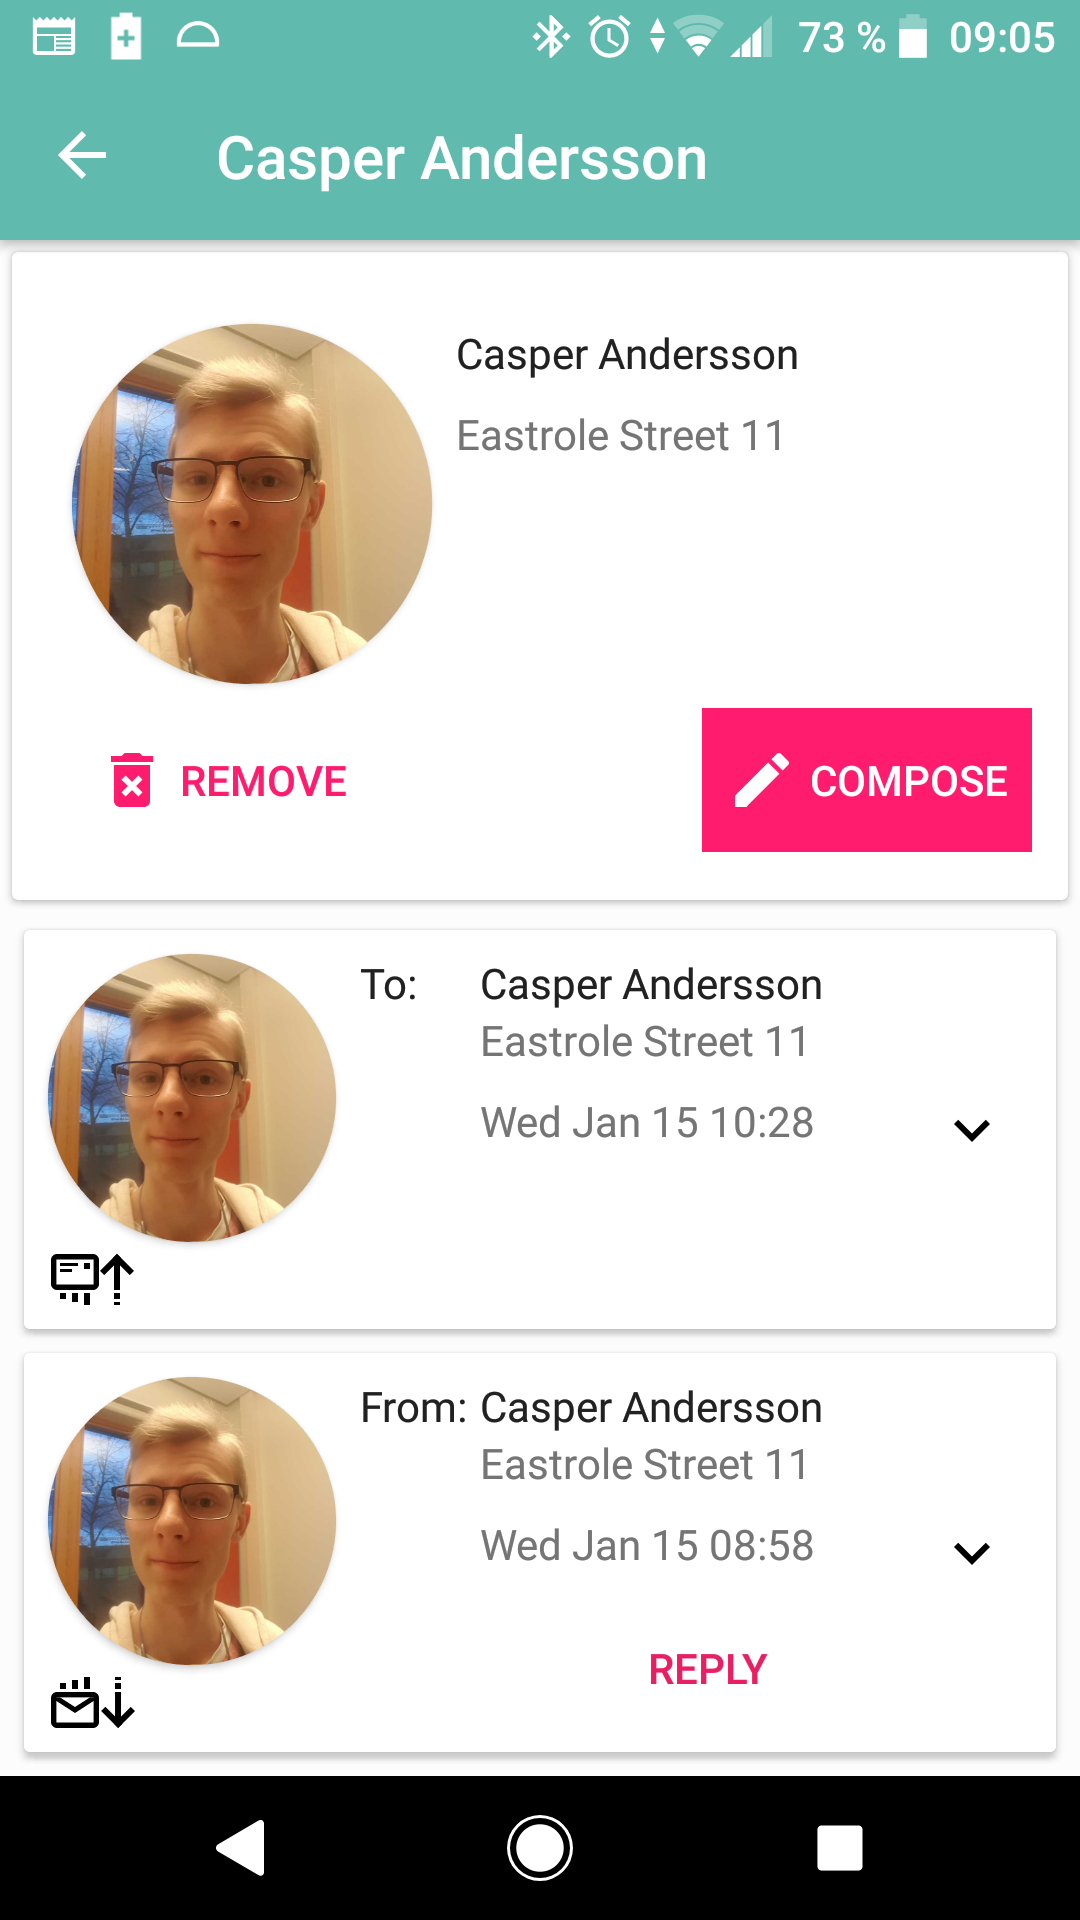
\includegraphics[width=\textwidth]{images/usertouser.png}
          \caption{The mail correspondence screen, where the letters and information for a specific user are shown with the option to read all received and sent letters. There are buttons to remove the contact, reply and compose a new letter.}
          \label{fig:usertouser}
        \end{minipage}
      \end{figure}

      \begin{figure}
        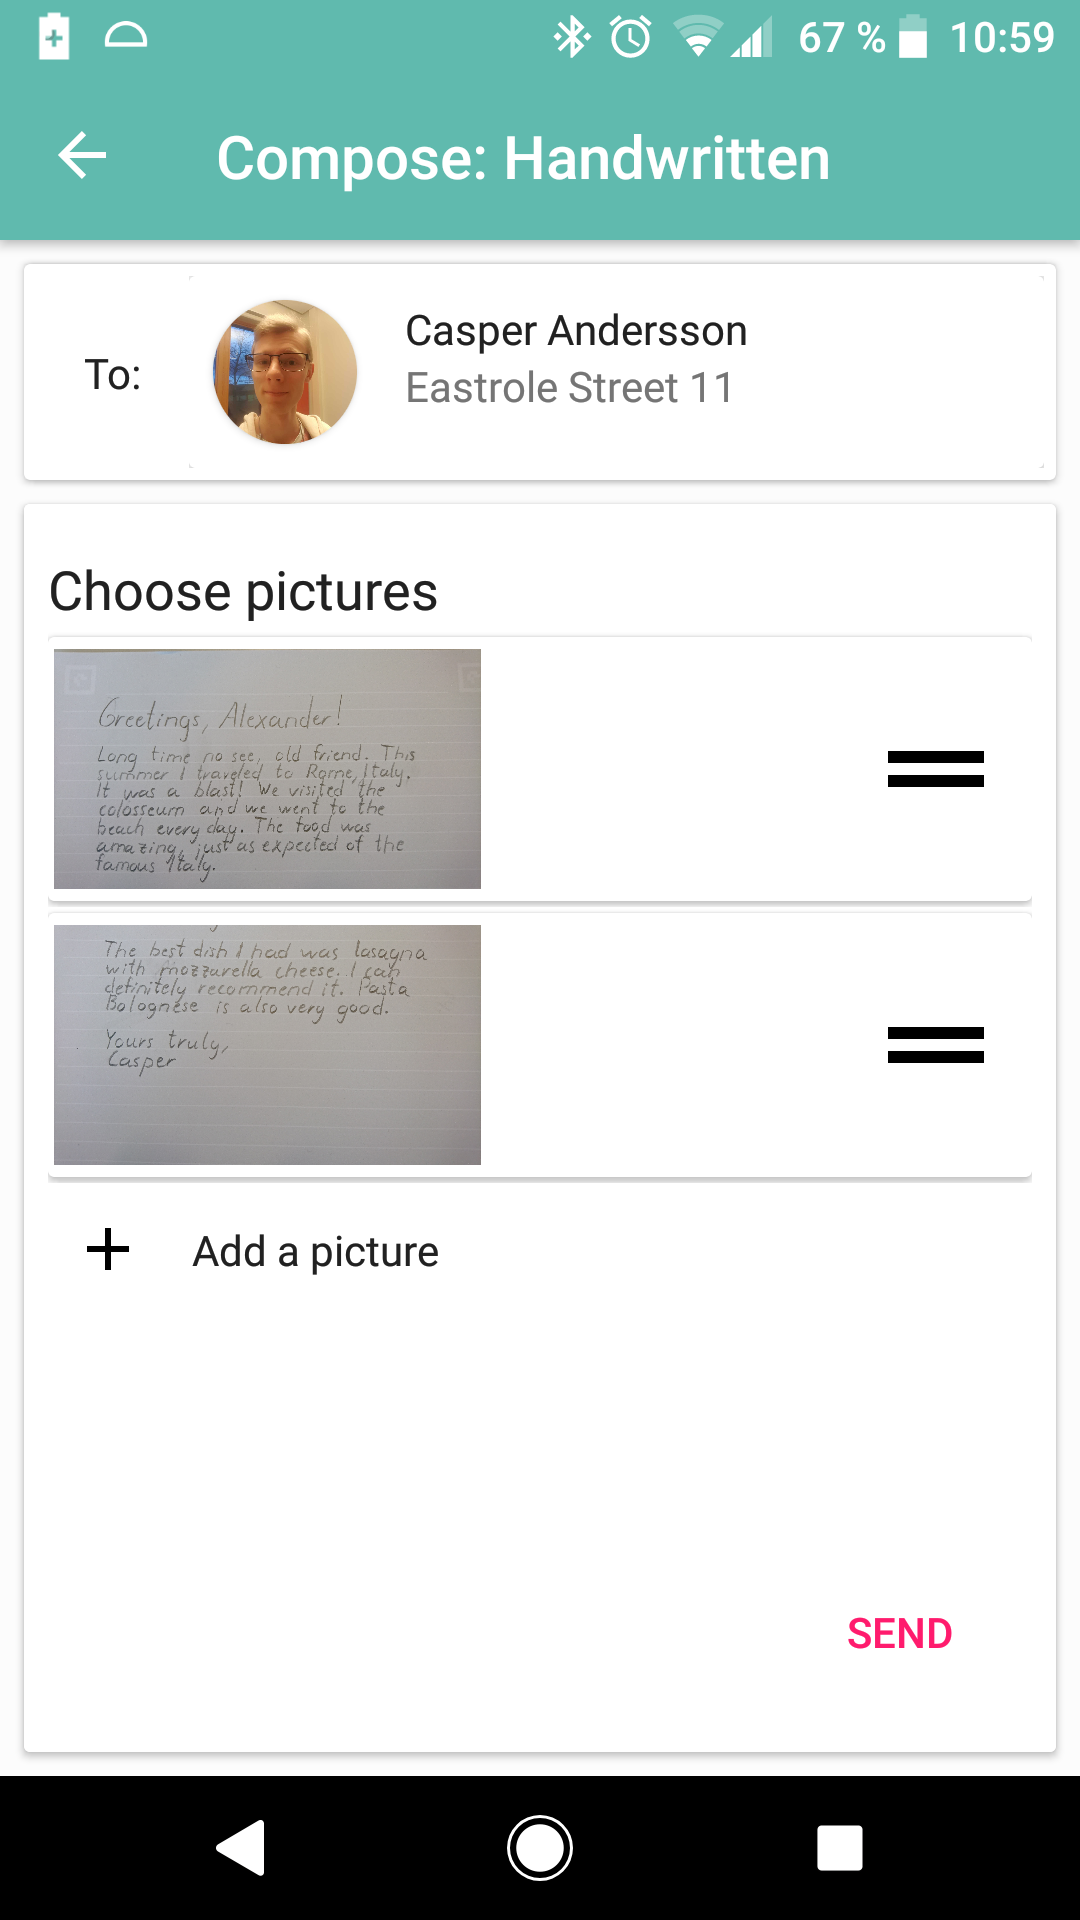
\includegraphics[width=5cm]{images/composepicagain.png}
        \Description{Compose view}
        \caption{Compose features a recipient bar that can be changed by touching it. The user can add pictures as well as rearrange them and the images can be removed by swiping.}
        \label{fig:compose}
      \end{figure}

    \subsection{Box}
      \textcolor{red}{[How the box screen is organized] [NG, PK]} \newline
      In the box (fig. \ref{fig:box}) messages are displayed. The tabs are filtered between all, received or sent messages. This is useful when the user wants to find a particular message. Pressing the profile picture of a contact opens your correspondence to that contact (fig. \ref{fig:usertouser}). Each letter can be expanded. The icon below the profile picture helps distinguish between received and sent letters. The icons are based on the google material icons\cite{materialicons} and have been modified.

    \subsection{Contacts}
      \textcolor{red}{[Contents of the contacts screen] [NG, PK]} \newline
      The contacts screen shows all your contacts (fig. \ref{fig:contacts}). When a contact card is pressed the user is taken to the correspondence screen for that user (fig. \ref{fig:usertouser}). The add button is conveniently placed in the lower right corner and when pressed, a popup is shown where the user can search for another user by their address. We wanted to allow the users to use their real name because it is more immersive when sending letters. That means that it cannot be unique. Therefore searching is done by address. We think it will be easier to share an address made up of two common words, rather than sharing a unique username like “catSlAyEr49xX”. We prevent users from finding other users that haven’t shared their address and reduce spam because the search term must be correctly written. Searching for “Effortmana Row” will not show a user with address “Effortmanager Row”. The downside is that users might expect common features such as searching by email or name. If we had more time we would have implemented that.

      \textcolor{red}{[How the contacts feature work] [CA]} \newline
      We decided to make contacts a one-way connection. Meaning if you add someone to your contacts they are not made aware that you added them, and will not receive a friend request. This imitates how a physical address/phone book works, and still does for the regular phone contacts, as opposed many apps that use a friend system.

    \subsection{Correspondence}
      \textcolor{red}{[How the correspondence screen works] [NG, PK]} \newline
      In the mail correspondence screen between two users, they can each see their contacts profile card and have the options to remove or send them a new letter (fig. \ref{fig:usertouser}). This screen was highly prioritized because it would allow users to view the letters to and from the same person. That makes it easy to re-read a conversation in order. When removing a user there is a pop-up confirmation screen to prevent accidentally removing a contact.

    \subsection{Compose}
      \textcolor{red}{[Compose fragment with picture letters] [NG, PK]} \newline
      Here we see that the user plans to send two images of their letter to their contact. The user can easily swap which contact to send these letters by pressing the recipient bar up top. They can also add more pictures and rearrange them dragging them up and down. If the user accidentally adds the wrong picture it can be removed by swiping left, the direction commonly used for this action in other apps.


  \section{Feedback and Improvements}
    \subsection{User feedback}
      \textcolor{red}{[Description of the received feedback] [EE]} \newline
      During the project presentation, we received feedback from testers. Most were regarding design choices in the user interface. Some users also suggested new features for future versions of the application.

      \textcolor{red}{[Feedback on the user interface] [EE, PK]} \newline
      During testing, some users thought it unclear what some parts of the user interface did. One tester found the button labels confusing when choosing what kind of letter to send. The labels were “Handwritten letter”, where a user can photograph or import a handwritten letter, and “Typed letter”, where the user can write a letter directly in the app. They interpreted the former as “Write by hand directly on the phone”. We had already anticipated this confusion by including descriptive icons for each button, but more thought can be put into the wording. A user thought the “your outbox is emptied:” text and the related timestamp were separated by a too-large space. We think this is because the spacing is more significant than alignment when mentally pairing visual artifacts\cite{lecturenotes-interaktion}. The reason for the large space was to separate the numerical data from the text to let the user gather information at a glance.
      Another tester found it difficult to read letters because they found the button that expands letters too small. They would prefer if the button was larger or if the entire card was clickable.

      \textcolor{red}{[Additional features suggested by the testers] [EE]} \newline
      The feedback we received included two additional features. One tester suggested allowing users to send postcards in addition to messages. The other suggested feature was having personal statistics. The app could show things like the number of messages sent/received and the total amount of time the user has spent on the app in the past week. The tester also suggested that the statistics could be shown at the end of the week as a weekly report.

    \subsection{Ideas for future development}
      \textcolor{red}{[Adding more settings] [CA]} \newline
      We would like to implement more settings. For example changing the password, profile picture and deleting your account. Changing your information is a feature that is present in almost every account-based application today and it’s something we should have as well. We briefly discussed a setting to only allow you to receive messages from people who are already in your contact list, which would prevent users from receiving any potential spam messages. Blocking users would also be a useful feature.

      \textcolor{red}{[Improving load times in the box screen] [CA, EE]} \newline
      When you open the box there is a noticeable delay if you have many messages, due to all the messages’ contents being loaded immediately. This could probably be solved by simply not loading the contents until you click on a message. It would instead put the delay on opening a message, but presumably not as significant. Currently, the messages are fetched each time the box screen is opened which results in a short delay. An optimization would be to keep the data used by the box in RAM when the box’s fragment is destroyed. The messages would then only need to be re-fetched when they receive another message. 

      \textcolor{red}{[Not storing all messages on the phone all the time] [CA, PK]} \newline
      Fetching all messages at once is not the optimal implementation. A lot of images will use a lot of storage space on the phone. This could become a problem in the long run. A solution to this is to only fetch the older letters when scrolling towards them. Older messages could be deleted regularly in background services. With this, we could also add an option in settings to clear the local message data to free up space and get rid of old messages that probably aren’t read often. Another helpful feature would be to load low-resolution versions of letters first and then dynamically update them with full resolution images.

      \textcolor{red}{[Plans for encrypted messages] [AA, PK]} \newline
      In the original vision of the application, we planned to encrypt all letters using private-public key cryptography. Letters would be encrypted using the senders private and public key in combination with the recipients public key. The recipient could then decrypt it using their private key and the sender's public key. This way not even a malicious host (us) could spy on the users’ correspondence. Since encryption was always planned to be a core feature in our application many parts were designed with support for encryption in mind. Due to time constraints, this feature had to be cut to implement other features.

    \subsection{Discussion}
      \textcolor{red}{[Did we achieve the initial specification?] [NG, PK]} \newline
      During the development process, we managed to reach almost all of the initial specifications we submitted to Afshin Ameri. In addition, we implemented several of the extra features. A user can send letters in two different ways: Written on paper or typed on the device. We also added a correspondence screen available for each contact. We implemented accounts, profiles with profile pictures and randomly generated addresses. However, at the end of the project, we lost focus on some of the minimum features from earlier. The features we failed to implement were the options to change the password and profile picture. We decided that they would be less essential when presenting the app compared to bug fixes and UI responsiveness.

      \textcolor{red}{[Reflection on how well we reached our goals] [NG, PK]} \newline
      The goals outlined in section [Objectives and goals] were reached. The application is stable without any persistently recurring crashes. We experienced one crash during demoing on an old device, but no data was lost. All data is backed up on the server and a saved draft state is maintained when composing a message. This makes us confident that atypical disruptions of the application’s activity are non-destructive. The application is scalable because it is deployed on a Microsoft Azure server. More users would simply mean paying for more server time. Additionally, user studies confirmed that the UI-structure functioned according to their expectations. 


      




  \bibliography{sources}

\end{document}